\documentclass[preprint,12pt]{elsarticle}

\usepackage{booktabs}
\usepackage{float}
\usepackage{amsmath}
\usepackage{amssymb}
\usepackage{array}
\usepackage{graphicx}
\usepackage{xcolor}
\usepackage{tikz}
\usepackage[hidelinks]{hyperref}
\usetikzlibrary{arrows.meta,positioning}
\newcolumntype{L}[1]{>{\raggedright\arraybackslash}p{#1}}
\emergencystretch=3em
\biboptions{numbers,sort&compress}

\journal{Data \& Knowledge Engineering}

\begin{document}
\begin{frontmatter}

\title{IAD-Risk: Risk-Aware Identity-Agenda Disentanglement for Scholarly Work Deduplication}
\author{Anonymous Authors}

\begin{abstract}
Scholarly entity matching must distinguish whether two records describe the same work, not merely whether they discuss the same research agenda. Modern scientific representations and pair classifiers often improve semantic matching, but a high semantic score can also connect different papers in the same task, benchmark, or citation community. This paper studies this failure mode as \emph{identity-agenda confusion} and proposes IAD-Risk, a risk-aware framework that separates identity evidence from agenda evidence before making merge decisions. IAD-Risk combines stratified data provenance, identity and agenda relation heads, and false-merge risk gating to prevent agenda-level hard negatives from entering automatic merge clusters. We evaluate the framework with IAD-Bench, a benchmark contract that separates DeepMatcher gold labels, SciRepEval/SciDocs-style proxy labels, and OpenAlex/OpenCitations silver hard negatives. In the Open-v2 evidence snapshot, single-space scientific representation baselines show HNFMR 0.790--0.999 on the full pair scope, whereas transformer-backed IAD-Risk variants report same-work F1=0.980 and HNFMR=0.000 on the held-out test scope. The results support a conservative conclusion: identity-agenda disentanglement is a practical mechanism for safer scholarly deduplication, while additional manual validation and broader source-heldout validation remain necessary before making broad method-ranking claims.
\end{abstract}

\begin{keyword}
scholarly entity matching \sep work deduplication \sep identity-agenda disentanglement \sep false-merge risk \sep provenance-aware evaluation \sep scientific document representation
\end{keyword}

\end{frontmatter}

\section{Introduction}

Scholarly knowledge systems rely on entity matching to decide whether multiple records describe the same scientific work. Digital libraries, literature review tools, citation graphs, recommender systems, and evidence synthesis pipelines all require stable work identities because a false merge can combine evidence from different papers and distort downstream analysis. This paper focuses on scholarly work deduplication: given two scholarly records with titles, abstracts, authors, venues, identifiers, topics, and citations, the system must decide whether the records can be safely merged as the same work.

The central challenge is that topical similarity is not identity evidence. Two papers can share a task, dataset, method family, citation neighborhood, or OpenAlex topic while making different contributions. Scientific representation models such as SPECTER and SciNCL are valuable because they bring related papers close in embedding space \citep{cohan2020specter,ostendorff2022scincl}, but the same behavior can create false-merge risk when a deduplication system treats semantic closeness as work identity. This failure is particularly important in scholarly settings because false merges are harder to repair than missed duplicates: once distinct papers are clustered as one work, citation counts, recommendation signals, and review evidence can be contaminated.

We formulate this failure mode as identity-agenda confusion. Identity refers to whether two records denote the same scholarly work. Agenda refers to whether two records discuss the same research problem, benchmark, method family, or citation community. Existing entity matching methods \citep{fellegi1969record,mudgal2018deep,li2020ditto} typically optimize pair classification, while scholarly document representation methods optimize semantic relatedness. Neither objective alone forces the model to learn that same-agenda pairs can be high-risk non-identities.

We propose IAD-Risk, a risk-aware identity-agenda disentanglement framework for scholarly work deduplication. IAD-Risk learns separate relation signals for same-work identity, same-agenda relatedness, and agenda-non-identity hard negatives, then derives a false-merge risk score from these signals. A pair is eligible for automatic merging only when identity evidence is sufficiently strong and agenda-non-identity risk remains below a merge threshold. This selective decision rule turns deduplication from a high-recall similarity problem into a risk-calibrated safety problem.

The paper makes three contributions. First, it defines identity-agenda confusion as a targeted failure mode in scholarly entity matching and introduces hard-negative false-merge rate as a safety metric. Second, it presents IAD-Bench, a provenance-aware benchmark contract that keeps gold, proxy, silver, and human-reviewed labels separate. Third, it evaluates IAD-Risk under the same pair contract used by representation and entity-matching baselines, while keeping clustering and artifact-audit interfaces as reproducible extensions rather than unsupported primary evidence. The current evidence supports targeted false-merge suppression under stratified evaluation; it does not support a broad method-ranking claim or a claim that silver labels replace human gold.

\begin{table}[H]
\caption{Contribution-evidence summary. The table states what each contribution is, which evidence supports it, and which stronger claim remains outside the current manuscript.}
\label{tab:contribution-evidence-summary}
\centering
\footnotesize
\setlength{\tabcolsep}{3pt}
\begin{tabular}{L{0.27\linewidth}L{0.33\linewidth}L{0.30\linewidth}}
\toprule
Contribution & Supporting evidence in this paper & Claim boundary \\
\midrule
Identity-agenda confusion as a scholarly deduplication failure mode. & Problem formulation, hard-negative false-merge rate, and Open-v2 hard-negative evidence. & Identifies a concrete safety failure mode, not a prevalence estimate for all scholarly corpora. \\
IAD-Bench as a provenance-aware pair contract. & Gold, proxy, silver, and manual-validation layers with label source, label strength, provenance, split, and hard-negative fields. & Defines an evaluation contract; proxy and silver labels are not human identity gold. \\
IAD-Risk as a risk-aware merge mechanism. & Open-v2 evidence snapshot with single-space baseline HNFMR 0.790--0.999 and held-out IAD-Risk same-work F1=0.980, HNFMR=0.000. & Supports targeted false-merge suppression, not a broad method-ranking claim. \\
\bottomrule
\end{tabular}
\end{table}

\section{Related Work}

Entity resolution research defines the broader pipeline in which scholarly deduplication is situated. Classical record linkage formalizes the decision of whether two records refer to the same entity \citep{fellegi1969record}, while modern surveys describe end-to-end entity resolution as a workflow involving blocking, matching, and clustering under scale and heterogeneity constraints \citep{christophides2020endtoend}. System work such as Magellan further emphasizes that practical entity matching requires sampling, labeling, debugging, workflow management, and production execution rather than only a matching function \citep{konda2016magellan}. IAD-Risk follows this pipeline view, but focuses on a specific safety gap in scholarly data: a pair can be highly related in topic or citation context while still being an unsafe merge.

Neural entity matching methods provide the closest algorithmic baselines for learning pair-level match decisions. DeepER represents tuples with neural distributed representations and supports blocking over learned tuple vectors \citep{ebraheem2018deeper}. DeepMatcher explores design choices for neural entity matching models \citep{mudgal2018deep}, and Ditto shows that transformer-based matching can benefit from pretraining, fine-tuning, and data augmentation \citep{li2020ditto}. RoBERTa-style pair encoders \citep{liu2019roberta} are therefore natural baselines for this paper. The distinction is that these methods usually optimize a same-entity classification objective, whereas IAD-Risk adds explicit same-agenda and agenda-non-identity heads so that semantic relatedness can become blocking evidence rather than merge evidence.

Scientific document representation methods are strong baselines because they intentionally capture citation, topical, and semantic relatedness. SPECTER uses citation-informed supervision to learn document-level scientific representations and introduced SciDocs as a document-level evaluation benchmark \citep{cohan2020specter}. SciNCL improves scientific representations with neighborhood contrastive learning \citep{ostendorff2022scincl}, and SciRepEval broadens scientific representation evaluation across classification, regression, ranking, and search while releasing the SPECTER2 model family \citep{singh2022scirepeval}. These methods are useful for candidate generation and relatedness scoring, but their optimization target is not conservative work identity. IAD-Risk therefore treats high scientific relatedness as a possible false-merge risk unless identity evidence is also strong.

Scientific language resources and open scholarly metadata make reproducible benchmark construction possible, but they do not remove the need for provenance-aware evaluation. SciBERT shows that domain-specific pretraining on scientific text improves scientific NLP tasks \citep{beltagy2019scibert}, and S2ORC provides metadata, abstracts, references, and structured full text for many open-access papers \citep{lo2019s2orc}. OpenAlex provides a large open index of scholarly works and concepts \citep{priem2022openalex}, while OpenCitations provides open citation data \citep{heibi2019opencitations}. IAD-Bench uses these resources to construct same-work, same-agenda, and agenda-non-identity evidence, but separates gold, proxy, and silver labels so that citation or topic proximity is never presented as human identity gold.

\begin{table}[H]
\caption{Positioning against the closest lines of work. IAD-Risk differs by treating agenda relatedness as a risk signal for merge decisions rather than as direct identity evidence.}
\label{tab:closest-work-positioning}
\centering
\footnotesize
\setlength{\tabcolsep}{3pt}
\begin{tabular}{L{0.18\linewidth}L{0.24\linewidth}L{0.26\linewidth}L{0.24\linewidth}}
\toprule
Line of work & Primary optimization target & Limitation for scholarly deduplication & IAD-Risk distinction \\
\midrule
End-to-end entity resolution systems & Blocking, matching, labeling, and deployment workflows. & Workflow abstractions do not separate topical relatedness from work identity. & Adds identity-agenda semantics and false-merge risk gates inside matching. \\
Neural entity matching & Pair-level same-entity classification from tuple or text encoders. & Strong text similarity can still link different papers in one agenda. & Trains same-work, same-agenda, and agenda-non-identity heads with provenance-aware masking. \\
Scientific document representations & Citation-informed or contrastive scientific relatedness embeddings. & Relatedness embeddings support retrieval but are unsafe as direct merge evidence. & Uses representation similarity as candidate and agenda evidence, then blocks risky merges. \\
Open scholarly metadata benchmarks & Public metadata, citation, and topic signals for scalable evaluation. & Topic or citation proximity is silver evidence, not human identity gold. & Reports gold, proxy, and silver strata separately and ties claims to label strength. \\
\bottomrule
\end{tabular}
\end{table}

\section{Problem Formulation}

Let $d_i$ and $d_j$ be two scholarly records. The target identity label $y^{I}_{ij}$ indicates whether the records describe the same scholarly work. The agenda label $y^{A}_{ij}$ indicates whether the records discuss a related research agenda. A hard negative is a pair with high agenda evidence but negative identity evidence:
\[
y^{A}_{ij}=1,\quad y^{I}_{ij}=0.
\]
This pair should not be merged even if the documents are semantically close.

We evaluate merge safety with hard-negative false-merge rate:
\[
\mathrm{HNFMR} = \frac{\#\{(i,j): \hat{m}_{ij}=1, y^{A}_{ij}=1, y^{I}_{ij}=0\}}{\#\{(i,j): y^{A}_{ij}=1, y^{I}_{ij}=0\}},
\]
where $\hat{m}_{ij}$ is the automatic merge decision. The goal is not only to maximize same-work F1, but also to control HNFMR under explicit evidence provenance.

\subsection{Notation and Relation Semantics}

Table~\ref{tab:notation} summarizes the notation used throughout the paper. The key distinction is that identity variables describe whether two records denote the same work, while agenda variables describe topical or citation-level relatedness. This distinction prevents a high relatedness score from being interpreted as direct merge evidence.

\begin{table}[H]
\caption{Notation and relation semantics. The paper uses separate symbols for identity, agenda relatedness, agenda-non-identity risk, and merge decisions.}
\label{tab:notation}
\centering
\small
\begin{tabular}{L{0.18\linewidth}L{0.34\linewidth}L{0.38\linewidth}}
\toprule
Symbol or field & Meaning & Role in evaluation \\
\midrule
$d_i,d_j$ & Two scholarly records. & Input pair for scoring and merge decisions. \\
$y^I_{ij}$ & Identity label: the records describe the same work. & Gold identity evidence when supported by the label source. \\
$y^A_{ij}$ & Agenda label: the records share a research agenda. & Proxy or silver relatedness evidence, not sufficient for merging. \\
$y^{ANI}_{ij}$ & Agenda-non-identity label. & Hard-negative supervision for pairs that are related but should not merge. \\
$p_{\mathrm{work}}$ & Predicted same-work probability. & Positive merge evidence. \\
$p_{\mathrm{agenda}}$ & Predicted agenda-relatedness probability. & Relatedness evidence that can increase risk when identity is weak. \\
$p_{\mathrm{ani}}$ & Predicted agenda-non-identity probability. & Direct risk evidence against automatic merging. \\
$p_{\mathrm{risk}}$ & Derived false-merge risk score. & Gate for rejecting or deferring risky pairs. \\
$\hat{m}_{ij}$ & Automatic merge decision. & Determines FMR and HNFMR. \\
label strength & Gold, proxy, silver, or manual validation layer. & Controls how a row can be used in training, evaluation, and claims. \\
\bottomrule
\end{tabular}
\end{table}

\section{IAD-Bench}

IAD-Bench is a benchmark contract for organizing scholarly pair evidence. It is not a claim that every label has the same evidential status. Each pair stores relation labels, expected identity labels, expected agenda labels, label source, label strength, provenance, split, and hard-negative level.

\begin{table}[H]
\caption{IAD-Bench label layers. Gold, proxy, and silver labels are reported separately to avoid overstating evidence strength.}
\label{tab:label-layers}
\centering
\footnotesize
\setlength{\tabcolsep}{3pt}
\begin{tabular}{L{0.15\linewidth}L{0.42\linewidth}L{0.33\linewidth}}
\toprule
Layer & Source & Use in this paper \\
\midrule
Gold & DeepMatcher / py\_entitymatching & Same-work identity evaluation \\
Proxy & SciRepEval / SciDocs-style proximity & Same-agenda analysis \\
Silver & OpenAlex / OpenCitations & Agenda-non-identity hard negatives \\
Manual validation & Independent human review & External validation target \\
\bottomrule
\end{tabular}
\end{table}

\subsection{Document Schema Contract}

IAD-Bench first standardizes each scholarly record before constructing pair evidence. Table~\ref{tab:iad-bench-document-schema} lists the document fields used by the manuscript. The contract keeps identity-bearing metadata, agenda-bearing metadata, and source provenance in one record so that downstream pair construction can be audited without redistributing raw third-party files.

\begin{table}[H]
\caption{IAD-Bench document schema contract. Missing values are represented by empty strings, empty arrays, or null values rather than by dropping required fields.}
\label{tab:iad-bench-document-schema}
\centering
\footnotesize
\setlength{\tabcolsep}{3pt}
\begin{tabular}{L{0.22\linewidth}L{0.38\linewidth}L{0.30\linewidth}}
\toprule
Field group & Required fields & Reviewer-facing role \\
\midrule
Record identity & \texttt{document\_id}, \texttt{source\_dataset} & Makes each standardized record traceable to its originating public source. \\
Text and authorship & \texttt{title}, \texttt{abstract}, \texttt{authors} & Provides the textual and author evidence used by identity and agenda features. \\
Bibliographic metadata & \texttt{year}, \texttt{venue}, \texttt{doi}, \texttt{arxiv\_id}, \texttt{openalex\_work\_id} & Supplies identifier and publication-context evidence for same-work decisions. \\
Agenda context & \texttt{topics}, \texttt{references} & Supplies topical and citation evidence used for same-agenda and hard-negative construction. \\
\bottomrule
\end{tabular}
\end{table}

\subsection{Pair Schema Contract}

IAD-Bench uses a pair schema that makes relation semantics and evidence strength auditable. Table~\ref{tab:iad-bench-pair-schema} lists the required fields used by the manuscript. The schema separates the binary same-work target from agenda relatedness, records the source and strength of each label, and keeps split and hard-negative metadata visible so that training, threshold selection, held-out reporting, and manual audit cannot be silently mixed.

\begin{table}[H]
\caption{IAD-Bench pair schema contract. The schema records identity labels, agenda labels, provenance, split assignment, and hard-negative status for each pair.}
\label{tab:iad-bench-pair-schema}
\centering
\footnotesize
\setlength{\tabcolsep}{3pt}
\begin{tabular}{L{0.24\linewidth}L{0.34\linewidth}L{0.32\linewidth}}
\toprule
Field group & Required fields & Reviewer-facing role \\
\midrule
Pair identity & \texttt{pair\_id}, \texttt{source\_document\_id}, \texttt{target\_document\_id} & Makes every row traceable to two standardized documents and prevents anonymous aggregate-only reporting. \\
Relation targets & \texttt{relation\_label}, \texttt{expected\_label}, \texttt{expected\_agenda\_label} & Separates same-work identity from agenda relatedness before metrics are computed. \\
Evidence source & \texttt{label\_source}, \texttt{label\_strength}, \texttt{label\_provenance} & Records whether a label is gold, proxy, silver, or human-audit evidence and what signals support it. \\
Evaluation control & \texttt{split}, \texttt{hard\_negative\_level} & Controls train/dev/test/audit use and identifies agenda-level hard negatives for HNFMR. \\
\bottomrule
\end{tabular}
\end{table}

The Open-v2 benchmark variant used in the core evidence combines 415 DeepMatcher gold pairs with 10,000 OpenAlex-derived silver hard negatives, producing 10,415 pair records over 1,737 documents. The DeepMatcher component provides same-work gold labels, while the OpenAlex component stresses same-agenda non-identity behavior. This design is intentionally conservative: OpenAlex and OpenCitations are used to expose false-merge risk, not to replace human gold.

\begin{table}[H]
\caption{Open-v2 benchmark composition used in the current evidence snapshot. The table separates identity evidence from hard-negative stress evidence before any metric is reported.}
\label{tab:openv2-composition}
\centering
\footnotesize
\setlength{\tabcolsep}{3pt}
\begin{tabular}{L{0.22\linewidth}L{0.10\linewidth}L{0.30\linewidth}L{0.28\linewidth}}
\toprule
Evidence stratum & Pair count & Evaluation role & Claim boundary \\
\midrule
DeepMatcher gold identity & 415 & Measures same-work matching ability. & Supports identity evaluation within the imported gold benchmark pairs. \\
OpenAlex and OpenCitations silver hard negatives & 10,000 & Stresses agenda-level false-merge behavior. & Supports hard-negative safety analysis, not human non-identity gold. \\
Open-v2 combined pair scope & 10,415 & Provides the shared pair contract for the reported evidence snapshot over 1,737 documents. & Supports the Open-v2 mechanism demonstration; broader source-heldout claims require additional artifacts. \\
\bottomrule
\end{tabular}
\end{table}

\section{Method}

\subsection{Overview}

IAD-Risk converts scholarly deduplication into selective risk-aware matching. Given a candidate pair, the model estimates identity, agenda, and agenda-non-identity signals, then derives a false-merge risk score. The final merge decision is made only when identity evidence exceeds a same-work threshold and risk evidence remains below blocking thresholds. Figure~\ref{fig:iad-risk-pipeline} summarizes the workflow.

\begin{figure}[H]
\centering
\small
\resizebox{\linewidth}{!}{%
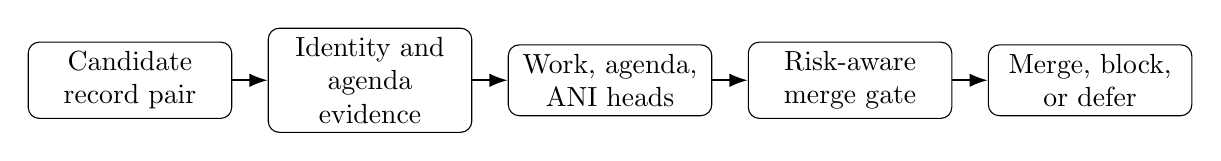
\begin{tikzpicture}[
  node distance=0.45cm,
  box/.style={draw, rounded corners, align=center, minimum height=0.8cm, text width=2.35cm},
  arrow/.style={-Latex, thick}
]
\node[box] (pair) {Candidate\\record pair};
\node[box, right=of pair] (evidence) {Identity and\\agenda evidence};
\node[box, right=of evidence] (heads) {Work, agenda,\\ANI heads};
\node[box, right=of heads] (gate) {Risk-aware\\merge gate};
\node[box, right=of gate] (output) {Merge, block,\\or defer};
\draw[arrow] (pair) -- (evidence);
\draw[arrow] (evidence) -- (heads);
\draw[arrow] (heads) -- (gate);
\draw[arrow] (gate) -- (output);
\end{tikzpicture}
}
\caption{IAD-Risk pipeline. The framework first separates identity evidence from agenda evidence, then predicts relation signals and derives a false-merge risk score before applying a conservative merge gate.}
\label{fig:iad-risk-pipeline}
\end{figure}

\subsection{Identity and Agenda Signals}

IAD-Risk separates the representation space into identity-oriented and agenda-oriented evidence. Identity evidence includes strong identifiers, near-duplicate titles, author overlap, year and venue agreement, and work-level metadata. Agenda evidence includes shared research topics, similar abstracts, citation neighborhoods, shared references, and scientific representation similarity. The separation is necessary because the same feature can have different meanings: high embedding similarity may indicate same work, but it may also indicate two different papers in the same research area.

\subsection{Multi-Task Relation Heads}

The model predicts three pair-level relation quantities: $p_{\mathrm{work}}$, $p_{\mathrm{agenda}}$, and $p_{\mathrm{ani}}$. The same-work head estimates identity. The same-agenda head estimates topical relatedness. The agenda-non-identity head detects pairs that are related but should not be merged. The false-merge risk score is then derived from these heads:
\[
p_{\mathrm{risk}}=\max\{p_{\mathrm{ani}},\ p_{\mathrm{agenda}}(1-p_{\mathrm{work}})\}.
\]
This construction makes the safety signal high when a pair is explicitly predicted as agenda-non-identity, or when it is agenda-related but lacks strong identity evidence.

\subsection{Risk Score Design Rationale}

$p_{\mathrm{risk}}$ is a conservative upper-envelope risk proxy for automatic merge decisions. The score increases monotonically with agenda-non-identity evidence through $p_{\mathrm{ani}}$, and it also increases when agenda evidence is high and identity evidence is weak through $p_{\mathrm{agenda}}(1-p_{\mathrm{work}})$. The max operator keeps either direct ANI evidence or indirect agenda-without-identity evidence sufficient to block automatic merging. This design matches the safety objective of the paper: a pair should defer rather than merge when either source of false-merge risk is high.

\begin{table}[H]
\caption{Risk score design rationale. The score is designed as a conservative merge gate, not as an unconditional probability of error.}
\label{tab:risk-score-rationale}
\centering
\footnotesize
\setlength{\tabcolsep}{3pt}
\begin{tabular}{L{0.24\linewidth}L{0.34\linewidth}L{0.32\linewidth}}
\toprule
Design element & Reviewer-facing rationale & Boundary \\
\midrule
$p_{\mathrm{ani}}$ term & Directly represents evidence that a related pair is not the same work. & Requires valid ANI supervision or artifact-backed hard-negative evidence. \\
$p_{\mathrm{agenda}}(1-p_{\mathrm{work}})$ term & Flags pairs that are topically related but lack corresponding identity support. & It is not a calibrated probability unless validated against held-out artifacts. \\
Max operator & Makes either risk pathway sufficient to block a merge. & Conservative blocking can increase deferrals and must be tuned to the application. \\
Threshold gate & Converts the risk proxy into a merge, block, or defer decision. & Threshold transfer must be rechecked under new source distributions. \\
\bottomrule
\end{tabular}
\end{table}

\subsection{Training Objective}

The learning objective combines identity, agenda, and agenda-non-identity supervision without treating every source as the same label type; the false-merge risk score is derived after the relation heads are estimated. For a pair $(i,j)$, the model minimizes
\[
\mathcal{L}_{ij} =
\lambda_w \mathrm{CE}(y^I_{ij}, p_{\mathrm{work}})
+ \lambda_a \mathrm{CE}(y^A_{ij}, p_{\mathrm{agenda}})
+ \lambda_n \mathrm{CE}(y^{ANI}_{ij}, p_{\mathrm{ani}}),
\]
where $\mathrm{CE}$ is binary cross-entropy and $\lambda_w,\lambda_a,\lambda_n$ control the contribution of each supervision channel. The key design choice is provenance-aware masking: a pair contributes only to the heads for which its label source is valid. For example, DeepMatcher pairs supervise same-work identity, whereas OpenAlex/OpenCitations silver hard negatives supervise agenda-non-identity risk without being promoted to human gold identity labels.

\subsection{Risk-Aware Merge Decision}

The merge policy is:
\[
\hat{m}_{ij}=1 \quad \mathrm{iff}\quad
p_{\mathrm{work}}\geq \tau_w,\quad
p_{\mathrm{ani}}<\tau_a,\quad
p_{\mathrm{risk}}<\tau_r,\quad
\mathrm{cannot\_link}_{ij}=0.
\]
This rule is deliberately selective. It can reject or defer high-risk pairs instead of forcing every semantically related pair into a binary match decision. The same decision interface also supports constrained union-find clustering, where cannot-link evidence prevents transitive false merges.

\subsection{Operational Complexity and Net Benefit}

IAD-Risk is appropriate when false merges are more costly than additional review. The additional cost comes from three relation heads and explicit threshold records, rather than from a new end-to-end clustering system. In an operational scholarly index, this cost is justified when a false merge can contaminate citation counts, literature-review evidence, or recommendation signals. In contrast, low-risk bulk cleanup tasks may prefer a simpler deduplication rule if occasional false merges have limited downstream effect.

\begin{table}[H]
\caption{Operational complexity and net-benefit boundary. The framework is intended for safety-sensitive scholarly identity decisions, not as a universal replacement for simple deduplication pipelines.}
\label{tab:operational-net-benefit}
\centering
\footnotesize
\setlength{\tabcolsep}{3pt}
\begin{tabular}{L{0.23\linewidth}L{0.33\linewidth}L{0.34\linewidth}}
\toprule
Operational item & Required practice & Net-benefit boundary \\
\midrule
Model complexity & Train and audit same-work, same-agenda, and ANI heads under one pair schema. & The net benefit is strongest in high-stakes scholarly indexes where false merges are costly. \\
Threshold governance & Select shared thresholds on validation evidence and record them in artifacts. & Thresholds are not tuned per pair or changed after test inspection. \\
Deferral policy & Record the deferral budget and manual-review capacity before deployment. & A high defer rate is acceptable only when review capacity exists. \\
Simple alternatives & Retain simple rules for low-risk bulk cleanup or identifier-only reconciliation. & IAD-Risk is not a universal replacement for simple deduplication pipelines. \\
\bottomrule
\end{tabular}
\end{table}

\subsection{Failure-Control Rationale}

IAD-Risk is designed as a failure-control framework rather than as another similarity scorer. Table~\ref{tab:failure-controls} summarizes how each design choice addresses a specific false-merge pathway. The table also states the remaining boundary for each control, because a safety mechanism should make its unsupported cases explicit.

\begin{table}[H]
\caption{Failure-control rationale of IAD-Risk. Each component targets a concrete way in which agenda-level similarity can be mistaken for work identity.}
\label{tab:failure-controls}
\centering
\small
\begin{tabular}{L{0.26\linewidth}L{0.34\linewidth}L{0.30\linewidth}}
\toprule
Failure pathway & Design response & Remaining boundary \\
\midrule
Topically close papers receive high semantic similarity. & Separate agenda evidence from identity evidence before the merge gate. & Requires the benchmark to include agenda-level hard negatives. \\
Silver metadata is treated as if it were human gold. & Preserve label strength and provenance, and mask supervision by valid label source. & Silver labels support stress testing, not exhaustive truth claims. \\
Pairwise errors contaminate clusters through transitivity. & Apply risk gating before constrained union-find and respect cannot-link evidence. & Cluster-level guarantees require complete cannot-link coverage. \\
Thresholds turn a classifier into an unsafe automatic merger. & Expose work, ANI, and risk thresholds and evaluate held-out merge decisions. & Threshold transfer should be rechecked under new source distributions. \\
Proxy labels are over-interpreted. & Keep proxy rows separate unless the label source supports the relation being evaluated. & Proxy rows remain non-human evidence even when reproducible. \\
\bottomrule
\end{tabular}
\end{table}

\subsection{Design Alternatives and Rejected Shortcuts}

Several simpler designs are plausible but unsafe for the claim made in this paper. Table~\ref{tab:design-alternatives} explains why IAD-Risk uses explicit identity, agenda, and agenda-non-identity signals instead of treating scholarly deduplication as ordinary semantic thresholding or a single pair-classification problem. The purpose of this comparison is not to dismiss these alternatives; some are strong baselines in the reported evidence. The point is that they do not expose the relation semantics needed to audit agenda-driven false merges.

\begin{table}[H]
\caption{Design alternatives considered during method design. Each rejected shortcut lacks an explicit mechanism for separating agenda relatedness from work identity or for auditing false-merge risk.}
\label{tab:design-alternatives}
\centering
\footnotesize
\setlength{\tabcolsep}{3pt}
\begin{tabular}{L{0.22\linewidth}L{0.28\linewidth}L{0.25\linewidth}L{0.15\linewidth}}
\toprule
Alternative & Why it is insufficient for this failure mode & IAD-Risk design response & Evidence boundary \\
\midrule
Tune a representation-similarity threshold. & High scientific relatedness can still connect different works in the same task, benchmark, or citation community. & Use representation similarity as candidate and agenda evidence, not direct merge evidence. & Supports false-merge-risk motivation, not a full retrieval benchmark. \\
Use one supervised pair classifier. & A strong classifier can reduce false merges but does not expose whether a positive score comes from identity or agenda evidence. & Predict same-work, same-agenda, and agenda-non-identity signals separately before gating. & RoBERTa remains a strong baseline; broad superiority is not claimed. \\
Use provenance as a model feature. & Source or split identifiers can create leakage and make held-out interpretation fragile. & Keep provenance as audit metadata and apply provenance-aware supervision masking. & Source-heldout claims require stronger source coverage. \\
Always force a binary merge decision. & Some pairs have related evidence but insufficient identity evidence, making automatic merging risky. & Emit merge, block, or defer through the risk-aware gate. & Defer behavior needs deployment-specific review policies. \\
Select thresholds after test results. & Post-hoc threshold choice can hide false-merge risk and inflate held-out conclusions. & Fix operating points before final reporting and require threshold artifacts for stronger claims. & Threshold stability needs a released grid and checksums. \\
\bottomrule
\end{tabular}
\end{table}

\subsection{Implementation Details}

The reported transformer variants use frozen scientific document encoders rather than end-to-end fine-tuning. For each candidate pair, the implementation builds three feature groups: identity features combine transformer distances with identifiers, author overlap, venue, and year signals; agenda features combine semantic similarity with topic and citation overlap; agenda-non-identity features add conflict indicators such as different identifiers and year conflict. The three relation heads are trained on the training split, and the merge policy exposes $\tau_w$, $\tau_a$, and $\tau_r$ as configurable thresholds. Unless a validation protocol overrides them, the implementation uses 0.5 for all three thresholds.

\subsection{Feature and Head Specification}

The implementation uses label provenance for supervision control, not as a predictive shortcut. Pair metadata such as label source, label strength, provenance, split, and hard-negative level are copied to prediction outputs for auditing, but they are excluded from the identity, agenda, and risk feature groups used by the relation heads. Table~\ref{tab:feature-head-specification} gives the implementation-level contract used by the reported transformer variants.

\begin{table}[H]
\caption{Feature and head specification for IAD-Risk transformer variants. Metadata fields are retained for auditing but are not used as model features.}
\label{tab:feature-head-specification}
\centering
\footnotesize
\setlength{\tabcolsep}{3pt}
\begin{tabular}{L{0.18\linewidth}L{0.27\linewidth}L{0.26\linewidth}L{0.19\linewidth}}
\toprule
Head or stage & Main input fields & Supervision or calculation & Output role \\
\midrule
Identity head & Transformer distances, title similarity, author overlap, first-author match, venue similarity, year match, DOI/arXiv/OpenAlex identifier agreement. & Same-work labels from valid identity evidence, with provenance-aware masking. & Estimates $p_{\mathrm{work}}$ as positive merge evidence. \\
Agenda head & Transformer cosine, title and venue similarity, OpenAlex-style topic overlap, reference Jaccard similarity, year-distance score. & Same-agenda proxy or silver evidence when the source supports agenda relatedness. & Estimates $p_{\mathrm{agenda}}$ as relatedness evidence, not direct merge evidence. \\
ANI risk head & Transformer distances, title and author signals, topic overlap, reference overlap, year conflict, identifier agreement, and different-identifier conflicts. & Agenda-non-identity hard negatives from valid hard-negative sources. & Estimates $p_{\mathrm{ani}}$ as direct blocking evidence. \\
Risk gate & $p_{\mathrm{work}}$, $p_{\mathrm{agenda}}$, $p_{\mathrm{ani}}$, $\tau_w$, $\tau_a$, $\tau_r$, and cannot-link flags. & Computes $p_{\mathrm{risk}}=\max\{p_{\mathrm{ani}},p_{\mathrm{agenda}}(1-p_{\mathrm{work}})\}$. & Emits merge, block, or defer decisions. \\
Audit metadata & Pair ID, source pair ID, label strength, label source, provenance, split, and hard-negative level. & Copied from pair records and result artifacts. & Supports artifact review; it is not a training feature. \\
\bottomrule
\end{tabular}
\end{table}

\section{Experiments}

\subsection{Dataset Construction and Evidence Strength}

Open-v2 is built by converting public scholarly metadata into a unified pair schema. DeepMatcher/py\_entitymatching records provide the same-work gold layer, while OpenAlex topics and OpenCitations-style citation signals provide agenda-level silver hard negatives. Each pair keeps its label strength, provenance, split, and hard-negative flag so that a gold identity result is never averaged with a silver stress-test result without being identified as such.

The benchmark therefore has two roles. The gold layer measures ordinary duplicate matching ability, and the silver hard-negative layer measures whether a system over-merges topically close but distinct papers. This separation is important for interpreting the results: a representation baseline can look useful for scientific retrieval while still being unsafe for automatic work identity merging.

\subsection{Split and Leakage Controls}

The evaluation protocol treats split assignment as part of the evidence contract rather than as a preprocessing detail. Each pair carries a split field, label strength, label source, relation label, provenance, and hard-negative level. Training uses only the declared training split, threshold selection uses validation evidence when available, and held-out metrics are reported only after the operating point has been fixed. Metadata fields that identify source, provenance, or split are retained for auditing but are excluded from model features.

\begin{table}[H]
\caption{Split and leakage controls used to interpret IAD-Bench results. The controls define what the current evidence supports and what stronger follow-up evidence would require.}
\label{tab:split-leakage-controls}
\centering
\footnotesize
\setlength{\tabcolsep}{3pt}
\begin{tabular}{L{0.24\linewidth}L{0.30\linewidth}L{0.34\linewidth}}
\toprule
Control & Manuscript role & Stronger evidence boundary \\
\midrule
Train/dev/test split field & Separates fitting, threshold selection, and held-out reporting. & Full numerical reproduction requires released prediction files, configs, and split summaries. \\
Unordered pair leakage guard & Detects whether the same document pair appears across multiple splits. & A blocked leakage audit prevents held-out claims until duplicate pair assignments are removed. \\
Label-stratum coverage audit & Checks whether gold, proxy, and silver evidence appear in the intended evaluation strata. & Missing strata must be reported as evidence gaps rather than averaged into a single score. \\
Source-heldout readiness audit & Tests whether relation labels have enough independent label sources for source-heldout claims. & Broad source generalization remains conditional until source-heldout coverage is defensible. \\
Topic-heldout readiness audit & Tests whether enough topics exist to reserve unseen-topic evaluation slices. & Cross-topic stability should not be claimed when topic coverage is insufficient. \\
\bottomrule
\end{tabular}
\end{table}

These controls reduce two common reviewer concerns. First, the model cannot gain accuracy from explicit provenance or split identifiers because those fields are audit metadata rather than predictive features. Second, a held-out result is interpreted only within the split and coverage regime that generated it. If a split-readiness audit blocks source-heldout or topic-heldout claims, the manuscript keeps the conclusion at the level of random-split or mechanism evidence instead of presenting it as broad generalization.

\subsection{Experimental Questions}

The experiments ask four questions. RQ1 tests whether IAD-Risk preserves same-work matching performance on gold labels. RQ2 tests whether it reduces false merges on agenda-level hard negatives. RQ3 examines whether the observed behavior is consistent with the proposed risk mechanism. RQ4 tests whether results remain interpretable under gold, proxy, and silver label strata.

\begin{table}[H]
\caption{Evaluation protocol. Each question is tied to a label stratum and a metric so that evidence strength is not mixed across sources.}
\label{tab:evaluation-protocol}
\centering
\small
\setlength{\tabcolsep}{3pt}
\begin{tabular}{L{0.08\linewidth}L{0.25\linewidth}L{0.17\linewidth}L{0.30\linewidth}}
\toprule
RQ & Evidence layer & Metric & Interpretation \\
\midrule
RQ1 & Gold identity pairs & Same-work F1 & Duplicate matching ability \\
RQ2 & Silver hard negatives & HNFMR & False-merge safety \\
RQ3 & Mechanism analysis & FMR and HNFMR & Role of risk signals \\
RQ4 & Gold/proxy/silver strata & Split metrics & Provenance-aware robustness \\
\bottomrule
\end{tabular}
\end{table}

\subsection{Evaluation Metrics}

Same-work F1 is computed on pairs whose identity labels come from the gold layer. Ordinary false-merge rate (FMR) is the fraction of non-identity pairs that the system marks for automatic merging. Hard-negative false-merge rate (HNFMR) is the same error measured only on agenda-level hard negatives, where topic or citation evidence is high but identity evidence is negative. Reporting both FMR and HNFMR separates general matching errors from the specific identity-agenda confusion that this paper studies.

\subsection{Threshold Selection and Uncertainty Reporting}

Threshold-sensitive systems are evaluated under a fixed selection protocol rather than by choosing the best test threshold after observing results. Merge thresholds are selected on validation evidence when validation rows are available; otherwise, the default implementation threshold is reported as a fixed operating point. The test split is then used only for final metric reporting. This protocol is necessary because a small threshold change can alter FMR and HNFMR more strongly than it alters same-work F1.

\begin{table}[H]
\caption{Threshold and uncertainty reporting protocol. The protocol separates what is required for the current main table from what is required for stronger follow-up claims.}
\label{tab:threshold-uncertainty-protocol}
\centering
\small
\begin{tabular}{L{0.23\linewidth}L{0.33\linewidth}L{0.34\linewidth}}
\toprule
Item & Reporting rule & Reviewer-facing purpose \\
\midrule
Merge thresholds & Record $\tau_w$, $\tau_a$, $\tau_r$, validation source, and fixed operating point. & Prevents post-hoc threshold selection on the test set. \\
Metric uncertainty & Report bootstrap intervals when prediction files and resampling logs are present in the artifact package. & Distinguishes stable effects from small numerical differences. \\
Risk metrics & Always report FMR and HNFMR with same-work F1. & Prevents a high F1 score from hiding unsafe hard-negative merges. \\
Ablation claims & Claim component causality only when no-risk-gate, no-ANI, and single-space variants are present. & Separates mechanism-consistent evidence from complete causal ablation evidence. \\
Artifact audit & Tie each numerical table to predictions, configs, logs, checksums, and commit identifiers. & Makes result-level reproduction possible without committing raw data. \\
\bottomrule
\end{tabular}
\end{table}

\subsection{Statistical Interpretation Boundary}

The reported Open-v2 numbers are point estimates for a fixed evidence snapshot, not statistical superiority estimates. Confidence intervals, significance tests, and model-ranking statements are intentionally withheld unless the released artifact package contains the exact prediction files, resampling logs, random seeds, and checksums used to compute them. In particular, an HNFMR value of 0.000 means that no hard-negative false merge was observed under the reported pair scope and operating point; it should not be read as proof of zero risk under all source distributions.

\begin{table}[H]
\caption{Statistical interpretation boundary for the Open-v2 evidence snapshot. The table states how reported numbers may be read before interval and significance artifacts are released.}
\label{tab:statistical-interpretation-boundary}
\centering
\footnotesize
\setlength{\tabcolsep}{3pt}
\begin{tabular}{L{0.22\linewidth}L{0.34\linewidth}L{0.34\linewidth}}
\toprule
Interpretation item & Current manuscript status & Required evidence before stronger claim \\
\midrule
Point estimates & Reported for the fixed Open-v2 scope, split, and operating points. & Prediction files, metric summaries, thresholds, and checksums for the same rows. \\
Confidence intervals & Not reported as primary evidence in the current manuscript. & \path{bootstrap_intervals} generated from the same prediction files, with command logs and random seeds. \\
Statistical significance & Not claimed for baseline ranking or model superiority. & Predefined tests, multiplicity handling, input artifacts, and reproducible analysis logs. \\
Zero HNFMR rows & Interpreted as no observed hard-negative false merge in the reported scope. & Larger source-heldout evidence and manual validation before any zero-risk wording. \\
Model ranking & Restricted to mechanism interpretation rather than a universal leaderboard. & Same-scope predictions, interval estimates, ablations, and manual-validation slice. \\
\bottomrule
\end{tabular}
\end{table}

\subsection{Operating Point Disclosure}

The main result table reports fixed operating points rather than post-hoc best test thresholds. Table~\ref{tab:operating-point-disclosure} summarizes how each row family obtains its decision field and operating point. Exact threshold values, selected validation sources, and command logs must be verified from the released artifact manifest before using the table for numerical reproduction.

\begin{table}[H]
\caption{Operating point disclosure for the Open-v2 result table. The table records how merge decisions are produced and what artifact is required for threshold audit.}
\label{tab:operating-point-disclosure}
\centering
\footnotesize
\setlength{\tabcolsep}{3pt}
\begin{tabular}{L{0.24\linewidth}L{0.24\linewidth}L{0.24\linewidth}L{0.18\linewidth}}
\toprule
Row family & Decision field & Operating point source & Audit requirement \\
\midrule
Representation cosine baselines & Cosine score threshold on scientific document embeddings. & Fixed baseline metric summary; threshold chosen before final test reporting. & Score file, metric summary, and threshold entry. \\
RoBERTa pair classifier & Pair match probability threshold. & Fixed pair-classifier metric summary under the same pair schema. & Prediction file, metric summary, and model log. \\
IAD-Risk transformer variants & $p_{\mathrm{work}}$, $p_{\mathrm{ani}}$, and $p_{\mathrm{risk}}$ under the risk gate. & Model configuration; default $\tau_w=\tau_a=\tau_r=0.5$ unless the artifact config records an override. & Prediction file, model JSON, thresholds, and checksums. \\
\bottomrule
\end{tabular}
\end{table}

\subsection{Threshold Sensitivity Evidence Status}

Threshold stability is treated as an audit requirement, not as an unsupported robustness claim. The current Open-v2 table reports fixed operating points and therefore supports the mechanism interpretation under those operating points. A stronger statement that the method is stable across thresholds would require a threshold grid computed from the same prediction files, predefined threshold ranges, metric summaries for each setting, and checksums in the released artifact manifest.

\begin{table}[H]
\caption{Threshold sensitivity evidence status. The table separates the current fixed-threshold claim from the additional artifact evidence required for threshold-stability claims.}
\label{tab:threshold-sensitivity-status}
\centering
\footnotesize
\setlength{\tabcolsep}{3pt}
\begin{tabular}{L{0.24\linewidth}L{0.33\linewidth}L{0.33\linewidth}}
\toprule
Audit item & Current manuscript status & Required artifact before stronger claim \\
\midrule
Fixed operating point & Reported through the operating-point disclosure table and tied to validation or default thresholds. & Configuration file recording $\tau_w$, $\tau_a$, $\tau_r$, baseline thresholds, and selection source. \\
Threshold grid & The threshold grid is not reported as primary evidence in the current manuscript. & Sensitivity table generated from the same prediction files over predefined threshold ranges. \\
Metric stability & Interpreted only for the reported operating points. & Per-threshold F1, FMR, HNFMR, pair counts, random seeds, and command logs. \\
Artifact manifest & Required for numerical audit but not included in Git. & Manifest and checksums that bind prediction files, summaries, thresholds, and code commit. \\
Reviewer interpretation & Supports fixed-threshold false-merge control, not threshold-stable ranking across all operating points. & Stronger threshold-stability wording only after the released artifact contains the grid evidence. \\
\bottomrule
\end{tabular}
\end{table}

\subsection{Baselines}

The main table reports two scientific representation cosine baselines and one supervised pair-classifier baseline: SciNCL cosine, SPECTER2 adapter cosine, and RoBERTa pair classification. These rows are evaluated through the same pair schema so that same-work F1 and hard-negative false-merge rate can be interpreted without mixing label strengths. Other repository baseline utilities are not used as primary manuscript evidence unless their metric summaries, prediction files, thresholds, and checksums are included in the released artifact package.

\subsection{Baseline Fairness Controls}

Baseline comparison is controlled through the pair contract rather than through a broad leaderboard claim. All baselines consume the same IAD-Bench pair records for the row scope being reported, and each row uses the same train/dev/test split field when training is required. Threshold-sensitive rows use validation-selected operating points before held-out reporting. All systems report same-work F1, FMR, and HNFMR from the same metric implementation.

\begin{table}[H]
\caption{Baseline fairness controls for the Open-v2 evidence snapshot. The controls make the reported comparison auditable while preserving the scope boundary of each row family.}
\label{tab:baseline-fairness-controls}
\centering
\footnotesize
\setlength{\tabcolsep}{3pt}
\begin{tabular}{L{0.23\linewidth}L{0.35\linewidth}L{0.32\linewidth}}
\toprule
Control & Application in the reported table & Reviewer-facing boundary \\
\midrule
Input rows & Baselines use the same IAD-Bench pair records within each reported row scope. & A stricter ranking requires same-scope released prediction files for all rows. \\
Split use & Trainable rows use the same train/dev/test split field; non-trainable representation rows are reported as fixed score baselines. & Different available scopes should not be read as a single leaderboard. \\
Threshold selection & Threshold-sensitive rows use validation-selected operating points or recorded fixed thresholds. & Post-hoc test-threshold selection is not used for the reported claims. \\
Feature boundary & Label source, provenance, and split identifiers are audit fields, not predictive features. & Provenance can explain evidence strength but cannot be used as a shortcut feature. \\
Metric implementation & All systems report same-work F1, FMR, and HNFMR from the same metric implementation. & Metric comparability does not remove the need for released predictions and checksums. \\
\bottomrule
\end{tabular}
\end{table}

\subsection{Implementation and Reproducibility}

All reported systems are evaluated through the same pair-level schema, split field, and metric implementation. Threshold-sensitive baselines select merge thresholds on validation evidence and are then evaluated on held-out evidence. The main metrics are same-work F1 on gold identity pairs, ordinary false-merge rate, and HNFMR on agenda-level hard negatives. Rows with different pair counts in Table~\ref{tab:openv2-results} should therefore be read as evidence for the same mechanism under different available result scopes, not as a single leaderboard.

The repository separates executable code from large data artifacts: raw third-party data remain outside Git, while processing scripts, fixture tests, schema contracts, and artifact-release rules remain version controlled. Reproduction starts from public sources, rebuilds IAD-Bench pair files through the documented CLI, and checks generated outputs with manifests and checksums. This organization is intended to make the main evidence reproducible without redistributing restricted or large source files. The supplementary material states the claim-evidence boundary for each major conclusion so that code-level reproducibility, artifact-level reproducibility, and manual-validation requirements are not conflated.

\subsection{Artifact Reproduction Protocol}

Because the repository does not redistribute large third-party data, reproducibility is divided into code-level reproduction and result-level artifact reproduction. Table~\ref{tab:reproduction-levels} defines what each level proves. The key principle is that small fixtures verify the processing contracts, while the full reported tables require either independently obtained public source files or a released artifact package with manifests and checksums.

\begin{table}[H]
\caption{Reproduction levels for auditing the repository and the reported evidence.}
\label{tab:reproduction-levels}
\centering
\small
\begin{tabular}{L{0.12\linewidth}L{0.38\linewidth}L{0.40\linewidth}}
\toprule
Level & Required input & Audit target \\
\midrule
L0 code check & Source tree, package environment, and manuscript scripts & Verify that the CLI, tests, public-release scan, and LaTeX build run in a clean environment. \\
L1 fixture rebuild & Public miniature fixtures under \texttt{tests/fixtures} & Verify that DeepMatcher, SciRepEval-style, OpenAlex-style, and IAD-Bench adapters produce the documented pair schema. \\
L2 public-source rebuild & Independently obtained public raw files from the cited sources & Rebuild derived IAD-Bench files with the documented data-processing commands and inspect label provenance. \\
L3 result audit & Released tables, predictions, logs, manifests, and checksums & Verify the numerical results reported in the manuscript against immutable artifact files. \\
\bottomrule
\end{tabular}
\end{table}

\subsection{Claim-Evidence Boundary for Result Interpretation}

The result interpretation follows a conservative claim-evidence boundary. Each reported conclusion must be tied to a label stratum, an output artifact, and a statement of what the evidence does not prove. This boundary is especially important because the benchmark combines gold identity pairs with proxy and silver stress-test evidence rather than treating all rows as one homogeneous test set.

\begin{table}[H]
\caption{Claim-evidence boundary used to interpret the reported results. Each claim class is paired with the supporting evidence and the claims that are intentionally not made.}
\label{tab:claim-evidence-boundary-main}
\centering
\small
\begin{tabular}{L{0.24\linewidth}L{0.30\linewidth}L{0.34\linewidth}}
\toprule
Claim class & Required support & Boundary not claimed \\
\midrule
Identity-agenda confusion is a concrete false-merge pathway. & Hard-negative false-merge rate on agenda-level silver pairs, compared with single-space scientific representation baselines. & A prevalence estimate for all scholarly corpora. \\
IAD-Risk reduces risky automatic merges in the reported setting. & Held-out Open-v2 IAD-Risk predictions, thresholds, metric summaries, and checksums. & A broad method-ranking claim or a claim that every source distribution is covered. \\
IAD-Bench supports provenance-aware evaluation. & Pair schema fields for relation type, label source, label strength, provenance, split, and hard-negative level. & A claim that proxy or silver rows are human-gold labels. \\
Repository-level reproduction is possible without committing raw data. & Public code, fixture tests, documented data-processing commands, manifest rules, and PDF build scripts. & Full numerical reproduction without public source files or a released artifact package. \\
\bottomrule
\end{tabular}
\end{table}

\subsection{Result Audit Trail}

Table~\ref{tab:openv2-results} should be read together with the artifact boundary in Table~\ref{tab:claim-evidence-boundary-main}. Each numerical row must be traceable to three audit objects: a prediction or score file, a metric summary produced from that file, and a checksum or manifest entry that fixes the artifact version. The Git repository verifies the schema, fixture rebuild, public-release boundary, manuscript build, and submission package, but it deliberately does not store raw third-party data, large model outputs, or full prediction files. Therefore the manuscript treats the Open-v2 table as a supported evidence snapshot and reserves full numerical reproduction for the released L3 artifact package.

\begin{table}[H]
\caption{Result artifact crosswalk for the Open-v2 evidence snapshot. Each row family in the main table has a required artifact path or manifest entry before it can be used for full numerical audit.}
\label{tab:result-artifact-crosswalk}
\centering
\footnotesize
\setlength{\tabcolsep}{3pt}
\begin{tabular}{L{0.22\linewidth}L{0.36\linewidth}L{0.32\linewidth}}
\toprule
Main-table evidence & Required artifact IDs & Reviewer audit purpose \\
\midrule
Open-v2 aggregate table & \path{open_v2_main_results}, \path{iad_bench_split_summary} & Verifies row scopes, pair counts, document counts, label strata, and metric columns. \\
Representation cosine baselines & \path{representation_baseline_scores}, \path{threshold_selection_logs} & Verifies SciNCL and SPECTER2 scores, threshold choices, and full-pair false-merge rates. \\
RoBERTa pair classifier & \path{supervised_baseline_predictions}, \path{threshold_selection_logs} & Verifies supervised baseline predictions under the same pair schema and fixed operating point. \\
IAD-Risk transformer variants & \path{iad_risk_predictions}, \path{threshold_selection_logs} & Verifies held-out predictions, relation-head scores, risk-gate decisions, thresholds, and split identifiers. \\
Optional stronger claims & \path{bootstrap_intervals}, \path{ablation_suite}, \path{manual_validation_slice} & Required only before claiming confidence intervals, component causality, or human label precision. \\
Threshold-stability claims & \path{threshold_sensitivity_grid}, \path{threshold_selection_logs} & Required only before claiming stability across operating points or threshold ranges. \\
\bottomrule
\end{tabular}
\end{table}

\subsection{Main Open-v2 Results}

\begin{table}[H]
\caption{Open-v2 evidence snapshot. Lower false-merge rate is better. Rows are reported only when supported by current output summaries; different pair counts indicate different available result scopes.}
\label{tab:openv2-results}
\centering
\small
\setlength{\tabcolsep}{3pt}
\begin{tabular}{L{0.36\linewidth}L{0.13\linewidth}rrr}
\toprule
System & Pairs & Same-work F1 $\uparrow$ & FMR $\downarrow$ & HNFMR $\downarrow$ \\
\midrule
SciNCL cosine & 10415 & 0.054 & 0.785 & 0.790 \\
SPECTER2 adapter cosine & 10415 & 0.044 & 0.999 & 0.999 \\
RoBERTa pair classifier & 10415 & 0.825 & 0.001 & 0.0001 \\
IAD-Risk transformer (SciNCL) & 1042 test & 0.980 & 0.001 & 0.000 \\
IAD-Risk transformer (SPECTER2) & 1042 test & 0.980 & 0.001 & 0.000 \\
\bottomrule
\end{tabular}
\end{table}

The Open-v2 evidence shows why identity-agenda disentanglement is necessary. Single-space scientific representation baselines preserve topical relatedness, but their merge threshold can produce high false-merge rates on OpenAlex silver hard negatives. IAD-Risk transformer variants keep high same-work F1 on the held-out Open-v2 test split while suppressing hard-negative false merges. RoBERTa pair classification is a strong baseline and narrows the gap substantially; therefore the paper does not make broad superiority claims. Instead, the main result is that relation heads plus an explicit risk score provide a transparent and controllable mechanism for false-merge suppression.

\subsection{Scope Compatibility of the Open-v2 Table}

The Open-v2 table is a scope-bounded evidence table, not a single leaderboard. Full pair-scope representation baselines test whether single-space scientific relatedness can over-merge agenda-level hard negatives across the available Open-v2 pairs. Held-out IAD-Risk rows test whether risk-gated transformer variants preserve same-work performance and suppress hard-negative merges under a split-based model-evaluation protocol. The valid comparison is therefore mechanistic: semantic relatedness alone is unsafe as automatic merge evidence, while explicit risk gating can block hard-negative merges in the reported held-out setting.

\begin{table}[H]
\caption{Scope compatibility for interpreting the Open-v2 evidence snapshot. The table states what each row family supports and which stronger comparison remains outside the current evidence.}
\label{tab:scope-compatibility}
\centering
\footnotesize
\setlength{\tabcolsep}{3pt}
\begin{tabular}{L{0.22\linewidth}L{0.20\linewidth}L{0.26\linewidth}L{0.22\linewidth}}
\toprule
Row family & Pair scope & Supported interpretation & Not supported \\
\midrule
Representation baselines & Full available Open-v2 pair scope. & Tests whether one-space scientific relatedness creates hard-negative merge risk. & A tuned neural pair-classifier ranking under the same held-out prediction file. \\
RoBERTa pair classifier & Full available Open-v2 pair scope. & Shows that a strong supervised pair classifier can suppress most hard-negative merges. & A component-level explanation of identity-agenda risk control. \\
IAD-Risk transformer variants & Held-out Open-v2 test scope. & Tests whether explicit identity, agenda, and ANI heads support risk-gated held-out decisions. & A general ranking over every baseline before all rows share the same released prediction scope. \\
Future stronger comparison & Same released prediction scope plus manual-validation slice. & Would support a stricter leaderboard and stronger label-precision claims. & A claim that this stronger comparison has already been completed by the current evidence snapshot. \\
\bottomrule
\end{tabular}
\end{table}

This scope boundary is important for review. The evidence is sufficient for the paper's conservative claim that identity-agenda disentanglement is a practical false-merge control mechanism. It is not sufficient for a broad ranking claim until all row families are regenerated with the same released prediction scope, threshold-selection logs, checksums, and an independent manual-validation slice.

\subsection{Extended Protocols and Boundaries}

Open-v3 and source-heldout protocols are retained as follow-up evaluation paths, not as additional result evidence in the current manuscript package. These protocols are useful because they specify how source-diverse and domain-diverse validation should be audited before broader claims are made. The manuscript therefore treats Open-v2 as the core mechanism demonstration and reserves Open-v3/source-heldout conclusions for a released artifact package that contains matched prediction scopes, threshold logs, checksums, and manual-validation evidence.

\section{Mechanism and Error Analysis}

The central mechanism question is whether false-merge control follows from explicit agenda-non-identity supervision and the derived risk score. The supported Open-v2 comparison gives mechanism-consistent evidence: single-space scientific representations can over-merge agenda-related hard negatives, while IAD-Risk makes agenda-non-identity evidence a direct blocking signal. This does not by itself establish a complete causal ablation. A complete ablation package must compare the full gate with variants that remove risk gating, remove agenda-non-identity supervision, or collapse identity and agenda evidence into one score.

\begin{table}[H]
\caption{Mechanism evidence and reviewer-facing interpretation. The table separates current evidence from ablation outputs that would be required for a stronger causal claim.}
\label{tab:mechanism-evidence}
\centering
\small
\begin{tabular}{L{0.26\linewidth}L{0.32\linewidth}L{0.32\linewidth}}
\toprule
Mechanism question & Current evidence & Reviewer-facing boundary \\
\midrule
Does topical relatedness create merge risk? & Representation baselines show high false-merge rates on OpenAlex silver hard negatives. & Supports a targeted failure mode, not a universal prevalence estimate. \\
Does explicit risk gating suppress hard-negative merges? & IAD-Risk transformer variants keep low HNFMR under the reported Open-v2 split. & Supports the reported contract and thresholds; transfer must be rechecked on new source mixes. \\
Is the gain caused by each IAD-Risk component? & The current manuscript reports mechanism-consistent HNFMR evidence. & A full causal claim requires ablations removing risk gating, ANI supervision, and single-space separation. \\
Can cluster-level contamination be eliminated? & The method supports cannot-link-aware constrained union-find. & Guarantees require sufficient cannot-link coverage and cluster-level artifact audits. \\
\bottomrule
\end{tabular}
\end{table}

The qualitative error taxonomy in Table~\ref{tab:error-taxonomy} states which failure cases the framework is designed to expose. The taxonomy is diagnostic rather than a measured error distribution unless a released artifact contains per-category annotations and adjudication logs. This distinction matters because some categories, such as version boundaries, require human judgment beyond metadata-derived silver evidence.

\begin{table}[H]
\caption{Error taxonomy for identity-agenda confusion. The table identifies the expected failure mode, the IAD-Risk control, and the audit evidence needed for stronger claims.}
\label{tab:error-taxonomy}
\centering
\footnotesize
\setlength{\tabcolsep}{3pt}
\begin{tabular}{L{0.22\linewidth}L{0.26\linewidth}L{0.24\linewidth}L{0.20\linewidth}}
\toprule
Error category & Typical source of confusion & IAD-Risk control & Stronger audit evidence \\
\midrule
Same task, different contribution & Papers share a benchmark, model family, or problem statement. & Agenda-non-identity head and HNFMR reporting. & Human-reviewed hard-negative slice with pair notes. \\
Citation-neighborhood neighbor & Papers share references or citation community but are distinct works. & Reference-overlap features contribute to agenda evidence, not direct merge evidence. & Citation-derived pair provenance and checksum-fixed predictions. \\
Version or extension boundary & Preprint, short paper, conference, and journal records are similar but may not be mergeable. & Conservative defer/block behavior when identity evidence is incomplete. & Manual adjudication with version-policy labels. \\
Identifier conflict & DOI, arXiv, or OpenAlex identifiers disagree despite text similarity. & Different-identifier conflicts enter the ANI risk head and cannot-link logic. & Identifier-resolution logs and conflict audit table. \\
Sparse metadata & Abstract, venue, author, or identifier fields are missing or noisy. & Merge requires positive identity evidence rather than semantic similarity alone. & Missing-field stratified metrics and per-source diagnostics. \\
\bottomrule
\end{tabular}
\end{table}

The error analysis emphasizes claim discipline. The current evidence supports identity-agenda risk modeling, stratified benchmark construction, and targeted false-merge suppression. It does not support claims that OpenAlex labels are human gold, that the system has broad domain superiority, that component-level ablations have already closed every mechanism question, or that manual annotation has already been completed.

\section{Limitations}

This study has four limitations. First, OpenAlex/OpenCitations hard negatives are silver labels, not human gold. They are useful for stress testing but must be reported separately from DeepMatcher gold labels. Second, SciRepEval/SciDocs-style proximity is a proxy for agenda relatedness, not proof of identity or non-identity. Third, source-heldout generalization remains mixed across model variants and should be expanded before making broad claims across scholarly domains. Fourth, an independently reviewed 500--1,000 pair validation slice would provide stronger evidence about label precision and difficult boundary cases; the supplementary material specifies the sampling, blinding, adjudication, and agreement-reporting protocol required before making stronger human-validation claims.

\section{Threats to Validity}

Construct validity depends on whether the label strata measure the intended relations. DeepMatcher pairs provide same-work identity evidence, but OpenAlex/OpenCitations hard negatives are silver stress-test pairs rather than manual non-identity gold. Internal validity depends on threshold selection and split separation; therefore threshold-sensitive systems must select thresholds on validation data and report held-out metrics. External validity is limited by the current source mix: the Open-v2 evidence supports the identity-agenda mechanism, while broader claims require more source-heldout and domain-diverse evaluation. Reproducibility depends on public data availability and stable processing scripts because the repository deliberately avoids redistributing large third-party data files.

Table~\ref{tab:validity-threats} summarizes the main validity risks and the safeguards used in the manuscript. The table is intentionally conservative: a mitigation reduces a specific reviewer concern, but it does not turn proxy or silver evidence into human-adjudicated truth.

\begin{table}[H]
\caption{Threats to validity and claim boundaries. Each risk is paired with the current mitigation and the remaining statement that should not be over-claimed.}
\label{tab:validity-threats}
\centering
\footnotesize
\setlength{\tabcolsep}{3pt}
\begin{tabular}{L{0.18\linewidth}L{0.24\linewidth}L{0.26\linewidth}L{0.22\linewidth}}
\toprule
Validity dimension & Main risk & Current mitigation & Remaining boundary \\
\midrule
Construct validity & Silver hard negatives may contain metadata noise. & Label strength is preserved; silver rows remain stress-test evidence. & Not a replacement for manual non-identity gold. \\
Internal validity & Threshold choice or split leakage can inflate metrics. & Operating points, split fields, and pair-leakage audits are required. & Numerical claims need released predictions and logs. \\
External validity & Open-v2 may not cover every source, topic, or version policy. & Claims are tied to Open-v2 and source-heldout evidence boundaries. & Broad deployment requires domain-diverse validation. \\
Conclusion validity & HNFMR evidence may be mistaken for full causality. & Ablation requirements precede component-level causal claims. & Complete causality requires no-gate, no-ANI, and single-space variants. \\
Reproducibility & Raw data and large predictions are not stored in Git. & Public commands, fixtures, manifests, checksums, and artifact rules are provided. & Full numeric audit requires L2/L3 artifacts. \\
Operational validity & Pair errors can propagate through transitive merges. & Risk gating and cannot-link-aware clustering are described. & Cluster guarantees need complete cannot-link coverage. \\
\bottomrule
\end{tabular}
\end{table}

\section{Conclusion}

IAD-Risk addresses a specific failure mode in scholarly entity matching: the tendency to confuse agenda similarity with work identity. By separating identity and agenda evidence and gating automatic merges through false-merge risk, the framework makes deduplication safer under stratified gold, proxy, and silver evaluation. The current evidence supports targeted false-merge suppression and a reproducible benchmark contract. Additional validation should expand independent manual review and source-heldout evaluation before the framework is used for broad method ranking across scholarly domains.

\section*{Data and Code Availability}

The source code, benchmark construction scripts, public-release checks, and manuscript build scripts are organized in the project repository. After installation, the reproducibility entry points include CLI commands for DeepMatcher conversion, proximity conversion in the SciRepEval style, weak-label construction from \mbox{OpenAlex} and OpenCitations, IAD-Bench assembly, stratification checks, source-bias diagnostics, baseline execution, IAD-Risk training, bootstrap analysis, and manuscript PDF generation.

Raw third-party data are not redistributed in the repository because the original sources have their own access conditions and licenses. The repository instead provides data-processing commands, schema contracts, fixture tests, and artifact-release guidance so that independent readers can reproduce the benchmark construction from public sources and verify generated artifacts through manifests, checksums, command logs, and fixed commit identifiers.

\section*{Ethics Statement}

This study uses public scholarly metadata and benchmark-style record linkage data. It does not involve human participants, clinical records, private user behavior, or animal experiments. Any future manual validation should be limited to scholarly record relation labels and should avoid collecting sensitive personal information.

\section*{Competing Interests}

The authors declare no competing interests.

\bibliographystyle{elsarticle-num}
\bibliography{../references}
\end{document}
